%%%%%%%%%%%%%%%%%%%%%%%%%%%%%%%%%%%%%%%%%
% Beamer Presentation
% LaTeX Template
% Version 1.0 (10/11/12)
%
% This template has been downloaded from:
% http://www.LaTeXTemplates.com
%
% License:
% CC BY-NC-SA 3.0 (http://creativecommons.org/licenses/by-nc-sa/3.0/)
%
%%%%%%%%%%%%%%%%%%%%%%%%%%%%%%%%%%%%%%%%%

%----------------------------------------------------------------------------------------
%   PACKAGES AND THEMES
%----------------------------------------------------------------------------------------

\documentclass[xcolor={x11names}]{beamer}

\mode<presentation> {

% The Beamer class comes with a number of default slide themes
% which change the colors and layouts of slides. Below this is a list
% of all the themes, uncomment each in turn to see what they look like.

%\usetheme{default}
%\usetheme{AnnArbor}
%\usetheme{Antibes}
%\usetheme{Bergen}
%\usetheme{Berkeley}
%\usetheme{Berlin}
%\usetheme{Boadilla}
%\usetheme{CambridgeUS}
%\usetheme{Copenhagen}
%\usetheme{Darmstadt}
%\usetheme{Dresden}
%\usetheme{Frankfurt}
%\usetheme{Goettingen}
%\usetheme{Hannover}
%\usetheme{Ilmenau}
%\usetheme{JuanLesPins}
%\usetheme{Luebeck}
\usetheme{Madrid}
%\usetheme{Malmoe}
%\usetheme{Marburg}
%\usetheme{Montpellier}
%\usetheme{PaloAlto}
%\usetheme{Pittsburgh}
%\usetheme{Rochester}
%\usetheme{Singapore}
%\usetheme{Szeged}
%\usetheme{Warsaw}

% As well as themes, the Beamer class has a number of color themes
% for any slide theme. Uncomment each of these in turn to see how it
% changes the colors of your current slide theme.

%\usecolortheme{albatross}
%\usecolortheme{beaver}
%\usecolortheme{beetle}
%\usecolortheme{crane}
%\usecolortheme{dolphin}
%\usecolortheme{dove}
%\usecolortheme{fly}
%\usecolortheme{lily}
%\usecolortheme{orchid}
%\usecolortheme{rose}
%\usecolortheme{seagull}
%\usecolortheme{seahorse}
%\usecolortheme{whale}
%\usecolortheme{wolverine}

%\setbeamertemplate{footline} % To remove the footer line in all slides uncomment this line
%\setbeamertemplate{footline}[page number] % To replace the footer line in all slides with a simple slide count uncomment this line

%\setbeamertemplate{navigation symbols}{} % To remove the navigation symbols from the bottom of all slides uncomment this line
}

\usepackage{graphicx} % Allows including images
\usepackage{booktabs} % Allows the use of \toprule, \midrule and \bottomrule in tables
\usepackage[utf8]{inputenc}
\usepackage[TS1,T1]{fontenc}
\usepackage{fourier, heuristica}
\usepackage{array, booktabs}
\usepackage{xcolor}
\usepackage{colortbl}
\usepackage{caption}
\usepackage{tikz}
\usetikzlibrary{positioning}
\DeclareCaptionFont{blue}{\color{LightSteelBlue3}}

% makes \addlegendimage available (typically only available within an
% axis environment):
\def\addlegendimage{\csname pgfplots@addlegendimage\endcsname}

\newcommand{\foo}{\color{LightSteelBlue3}\makebox[0pt]{\textbullet}\hskip-0.5pt\vrule width 1pt\hspace{\labelsep}}
%\newcommand{\foo}{\color{blue}\makebox[0pt]{\textbullet}\hskip-0.5pt\vrule width 1pt\hspace{\labelsep}}

%----------------------------------------------------------------------------------------
%   TITLE PAGE
%----------------------------------------------------------------------------------------

\title[Map Fusion for Collaborative UAV SLAM]{Progress report\\Map Fusion for Collaborative UAV SLAM} % The short title appears at the bottom of every slide, the full title is only on the title page

\author{Andreas Ziegler} % Your name
\institute[V4RL@ETHZ] % Your institution as it will appear on the bottom of every slide, may be shorthand to save space
{
  
\includegraphics[scale=0.4]{../V4RLLogo} \\ETH Zurich \\ % Your institution for the title page
\medskip
\textit{anziegle@ethz.ch} % Your email address
}
\date{\today} % Date, can be changed to a custom date

\begin{document}

\begin{frame}
\titlepage % Print the title page as the first slide
\end{frame}

%\begin{frame}
%\frametitle{Overview} % Table of contents slide, comment this block out to remove it
%\tableofcontents % Throughout your presentation, if you choose to use \section{} and \subsection{} commands, these will automatically be printed on this slide as an overview of your presentation
%\end{frame}

%----------------------------------------------------------------------------------------
%   PRESENTATION SLIDES
%----------------------------------------------------------------------------------------

%------------------------------------------------
%\section{What I did so far} % Sections can be created in order to organize your presentation into discrete blocks, all sections and subsections are automatically printed in the table of contents as an overview of the talk
%------------------------------------------------

%\subsection{Subsection Example} % A subsection can be created just before a set of slides with a common theme to further break down your presentation into chunks

\begin{frame}
\frametitle{Recent steps}
\begin{itemize}
  \item Started implementing a first approach
  \item Realized this approach doesn't suite the g2o framework.
\end{itemize}
\end{frame}

%------------------------------------------------

\begin{frame}
\frametitle{A first approach}
  \only<1> {
    \begin{block}{Idea}
      Use the map points of multiple matches the calculate a better transformation
    \end{block}
    \begin{center}
    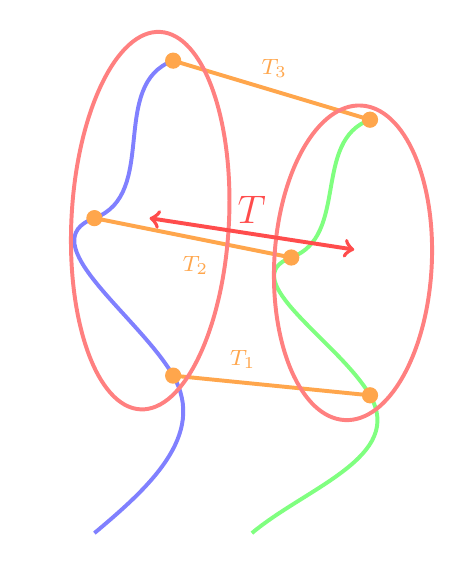
\begin{tikzpicture}
      \coordinate (A1) at (0, 0);
      \coordinate (B1) at (1, 2.0);
      \coordinate (C1) at (0, 4);
      \coordinate (D1) at (1, 6);

      \coordinate (A2) at (2, 0);
      \coordinate (B2) at (3.5, 1.75);
      \coordinate (C2) at (2.5, 3.5);
      \coordinate (D2) at (3.5, 5.25);

      \node at (A1) {};
      \node at (C1) {};
      \node at (D1) {};

      \node at (A2) {};
      \node at (C2) {};
      \node at (D2) {};

      \draw [blue!50, line width=0.05cm] (A1) to [out=40, in=-60] (B1);
      \draw [blue!50, line width=0.05cm] (B1) to [out=120, in=200] (C1);
      \draw [blue!50, line width=0.05cm] (C1) to [out=20, in=200] (D1);

      \draw [green!50, line width=0.05cm] (A2) to [out=40, in=-60] (B2);
      \draw [green!50, line width=0.05cm] (B2) to [out=120, in=200] (C2);
      \draw [green!50, line width=0.05cm] (C2) to [out=20, in=200] (D2);

      \node [fill=orange!70, circle,inner sep=2pt, text width=0.1mm] at (B1) {};
      \node [fill=orange!70, circle,inner sep=2pt, text width=0.1mm] at (B2) {};
      \node [fill=orange!70, circle,inner sep=2pt, text width=0.1mm] at (C1) {};
      \node [fill=orange!70, circle,inner sep=2pt, text width=0.1mm] at (C2) {};
      \node [fill=orange!70, circle,inner sep=2pt, text width=0.1mm] at (D1) {};
      \node [fill=orange!70, circle,inner sep=2pt, text width=0.1mm] at (D2) {};
      \draw [orange!70, line width=0.05cm] (B1) to (B2);
      \draw [orange!70, line width=0.05cm] (C1) to (C2);
      \draw [orange!70, line width=0.05cm] (D1) to (D2);
      \node [orange!70, right=of B1, xshift=-0.4cm, yshift=0.2cm] {\footnotesize$\text{T}_1$};
      \node [orange!70, right=of C1, yshift=-0.6cm] {\footnotesize$\text{T}_2$};
      \node [orange!70, right=of D1, yshift=-0.1cm] {\footnotesize$\text{T}_3$};

      \draw (0.5, 4) [red!50, line width=0.05cm, rotate=-3] ellipse (1.0cm and 2.4cm);
      \draw (3.1, 3.6) [red!50, line width=0.05cm, rotate=-3] ellipse (1.0cm and 2.0cm);
      \draw [red!70, line width=0.05cm, <->] (0.7, 4) to (3.3, 3.6);
      \node [red!70, yshift=0.1cm] at (2, 4)   (a) {\Large$\text{T}$};

    \end{tikzpicture}
    \end{center}
  }
  \only<2> {
    \begin{block}{Problem}
      To get one transformation out of the optimization over multiple matches, two ``virtual'' keyframes would have to be created, which have a plane, in which all the observed map points could be projected into.
    \end{block}
    \begin{center}
    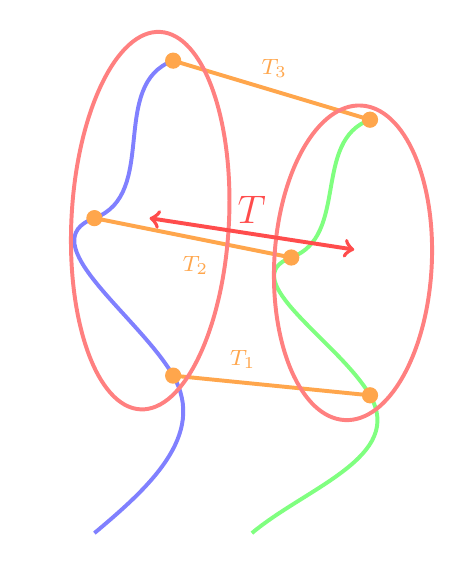
\begin{tikzpicture}
      \coordinate (A1) at (0, 0);
      \coordinate (B1) at (1, 2.0);
      \coordinate (C1) at (0, 4);
      \coordinate (D1) at (1, 6);

      \coordinate (A2) at (2, 0);
      \coordinate (B2) at (3.5, 1.75);
      \coordinate (C2) at (2.5, 3.5);
      \coordinate (D2) at (3.5, 5.25);

      \node at (A1) {};
      \node at (C1) {};
      \node at (D1) {};

      \node at (A2) {};
      \node at (C2) {};
      \node at (D2) {};

      \draw [blue!50, line width=0.05cm] (A1) to [out=40, in=-60] (B1);
      \draw [blue!50, line width=0.05cm] (B1) to [out=120, in=200] (C1);
      \draw [blue!50, line width=0.05cm] (C1) to [out=20, in=200] (D1);

      \draw [green!50, line width=0.05cm] (A2) to [out=40, in=-60] (B2);
      \draw [green!50, line width=0.05cm] (B2) to [out=120, in=200] (C2);
      \draw [green!50, line width=0.05cm] (C2) to [out=20, in=200] (D2);

      \node [fill=orange!70, circle,inner sep=2pt, text width=0.1mm] at (B1) {};
      \node [fill=orange!70, circle,inner sep=2pt, text width=0.1mm] at (B2) {};
      \node [fill=orange!70, circle,inner sep=2pt, text width=0.1mm] at (C1) {};
      \node [fill=orange!70, circle,inner sep=2pt, text width=0.1mm] at (C2) {};
      \node [fill=orange!70, circle,inner sep=2pt, text width=0.1mm] at (D1) {};
      \node [fill=orange!70, circle,inner sep=2pt, text width=0.1mm] at (D2) {};
      \draw [orange!70, line width=0.05cm] (B1) to (B2);
      \draw [orange!70, line width=0.05cm] (C1) to (C2);
      \draw [orange!70, line width=0.05cm] (D1) to (D2);
      \node [orange!70, right=of B1, xshift=-0.4cm, yshift=0.2cm] {\footnotesize$\text{T}_1$};
      \node [orange!70, right=of C1, yshift=-0.6cm] {\footnotesize$\text{T}_2$};
      \node [orange!70, right=of D1, yshift=-0.1cm] {\footnotesize$\text{T}_3$};

      \draw (0.5, 4) [red!50, line width=0.05cm, rotate=-3] ellipse (1.0cm and 2.4cm);
      \draw (3.1, 3.6) [red!50, line width=0.05cm, rotate=-3] ellipse (1.0cm and 2.0cm);
      \draw [red!70, line width=0.05cm, <->] (0.7, 4) to (3.3, 3.6);
      \node [red!70, yshift=0.1cm] at (2, 4)   (a) {\Large$\text{T}$};
    \end{tikzpicture}
    \end{center}
  }
\end{frame}

%------------------------------------------------

\begin{frame}
\frametitle{Recent steps}
\begin{itemize}
  \item Started implementing a first approach
  \item Realized this approach doesn't suite the g2o framework.
  \item Started with a new approach
\end{itemize}
\end{frame}

%------------------------------------------------

\begin{frame}
\frametitle{The new approach}
\only<1>{
  \begin{enumerate}
    \item Find $n$ keyframe matches
    \item Merge the two maps with the transformation of one of the keyframe matches
    \item Fuse map points in the $n-1$ keyframe matches
    \item Pose graph optimization over essential graph
    \item Global bundle adjustment
  \end{enumerate}
}
\only<2>{
  Find $n$ keyframe matches
  \begin{center}
  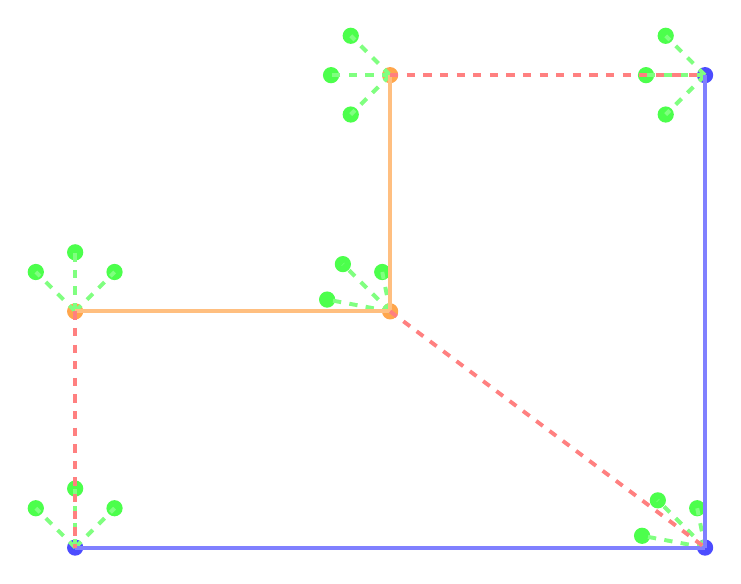
\begin{tikzpicture}
    \coordinate (A1) at (0, 3);
    \coordinate (A1MP1) at (-0.5, 3.5);
    \coordinate (A1MP2) at (0, 3.75);
    \coordinate (A1MP3) at (0.5, 3.5);

    \coordinate (B1) at (4, 3);
    \coordinate (B1MP1) at (3.2, 3.15);
    \coordinate (B1MP2) at (3.4, 3.6);
    \coordinate (B1MP3) at (3.9, 3.5);

    \coordinate (C1) at (4, 6);
    \coordinate (C1MP1) at (3.5, 6.5);
    \coordinate (C1MP2) at (3.25, 6.0);
    \coordinate (C1MP3) at (3.5, 5.5);

    \coordinate (A2) at (0, 0);
    \coordinate (A2MP1) at (-0.5, 0.5);
    \coordinate (A2MP2) at (0, 0.75);
    \coordinate (A2MP3) at (0.5, 0.5);

    \coordinate (B2) at (8, 0);
    \coordinate (B2MP1) at (7.2, 0.15);
    \coordinate (B2MP2) at (7.4, 0.6);
    \coordinate (B2MP3) at (7.9, 0.5);

    \coordinate (C2) at (8, 6);
    \coordinate (C2MP1) at (7.5, 6.5);
    \coordinate (C2MP2) at (7.25, 6.0);
    \coordinate (C2MP3) at (7.5, 5.5);

    \node [fill=orange!70, circle,inner sep=2pt, text width=0.1mm] at (A1) {};
    \node [fill=green!70, circle,inner sep=2pt, text width=0.1mm] at (A1MP1) {};
    \node [fill=green!70, circle,inner sep=2pt, text width=0.1mm] at (A1MP2) {};
    \node [fill=green!70, circle,inner sep=2pt, text width=0.1mm] at (A1MP3) {};
    \draw [green!50, dashed, line width=0.05cm] (A1) to (A1MP1);
    \draw [green!50, dashed, line width=0.05cm] (A1) to (A1MP2);
    \draw [green!50, dashed, line width=0.05cm] (A1) to (A1MP3);

    \node [fill=orange!70, circle, inner sep=2pt, text width=0.1mm] at (B1) {};
    \node [fill=green!70, circle, inner sep=2pt, text width=0.1mm] at (B1MP1) {};
    \node [fill=green!70, circle, inner sep=2pt, text width=0.1mm] at (B1MP2) {};
    \node [fill=green!70, circle, inner sep=2pt, text width=0.1mm] at (B1MP3) {};
    \draw [green!50, dashed, line width=0.05cm] (B1) to (B1MP1);
    \draw [green!50, dashed, line width=0.05cm] (B1) to (B1MP2);
    \draw [green!50, dashed, line width=0.05cm] (B1) to (B1MP3);

    \node [fill=orange!70, circle,inner sep=2pt, text width=0.1mm] at (C1) {};
    \node [fill=green!70, circle, inner sep=2pt, text width=0.1mm] at (C1MP1) {};
    \node [fill=green!70, circle, inner sep=2pt, text width=0.1mm] at (C1MP2) {};
    \node [fill=green!70, circle, inner sep=2pt, text width=0.1mm] at (C1MP3) {};
    \draw [green!50, dashed, line width=0.05cm] (C1) to (C1MP1);
    \draw [green!50, dashed, line width=0.05cm] (C1) to (C1MP2);
    \draw [green!50, dashed, line width=0.05cm] (C1) to (C1MP3);

    \node [fill=blue!70, circle,inner sep=2pt, text width=0.1mm] at (A2) {};
    \node [fill=green!70, circle,inner sep=2pt, text width=0.1mm] at (A2MP1) {};
    \node [fill=green!70, circle,inner sep=2pt, text width=0.1mm] at (A2MP2) {};
    \node [fill=green!70, circle,inner sep=2pt, text width=0.1mm] at (A2MP3) {};
    \draw [green!50, dashed, line width=0.05cm] (A2) to (A2MP1);
    \draw [green!50, dashed, line width=0.05cm] (A2) to (A2MP2);
    \draw [green!50, dashed, line width=0.05cm] (A2) to (A2MP3);

    \node [fill=blue!70, circle,inner sep=2pt, text width=0.1mm] at (B2) {};
    \node [fill=green!70, circle,inner sep=2pt, text width=0.1mm] at (B2MP1) {};
    \node [fill=green!70, circle,inner sep=2pt, text width=0.1mm] at (B2MP2) {};
    \node [fill=green!70, circle,inner sep=2pt, text width=0.1mm] at (B2MP3) {};
    \draw [green!50, dashed, line width=0.05cm] (B2) to (B2MP1);
    \draw [green!50, dashed, line width=0.05cm] (B2) to (B2MP2);
    \draw [green!50, dashed, line width=0.05cm] (B2) to (B2MP3);

    \node [fill=blue!70, circle,inner sep=2pt, text width=0.1mm] at (C2) {};
    \node [fill=green!70, circle, inner sep=2pt, text width=0.1mm] at (C2MP1) {};
    \node [fill=green!70, circle, inner sep=2pt, text width=0.1mm] at (C2MP2) {};
    \node [fill=green!70, circle, inner sep=2pt, text width=0.1mm] at (C2MP3) {};
    \draw [green!50, dashed, line width=0.05cm] (C2) to (C2MP1);
    \draw [green!50, dashed, line width=0.05cm] (C2) to (C2MP2);
    \draw [green!50, dashed, line width=0.05cm] (C2) to (C2MP3);

    \draw [orange!50, line width=0.05cm] (A1) to (B1);
    \draw [orange!50, line width=0.05cm] (B1) to (C1);
    \draw [blue!50, line width=0.05cm] (A2) to (B2);
    \draw [blue!50, line width=0.05cm] (B2) to (C2);

    \draw [red!50, line width=0.05cm, dashed] (A1) to (A2);
    \draw [red!50, line width=0.05cm, dashed] (B1) to (B2);
    \draw [red!50, line width=0.05cm, dashed] (C1) to (C2);
  \end{tikzpicture}
  \end{center}
}
\only<3>{
  Merge the two maps with the transformation of one of the keyframe matches
  \begin{center}
  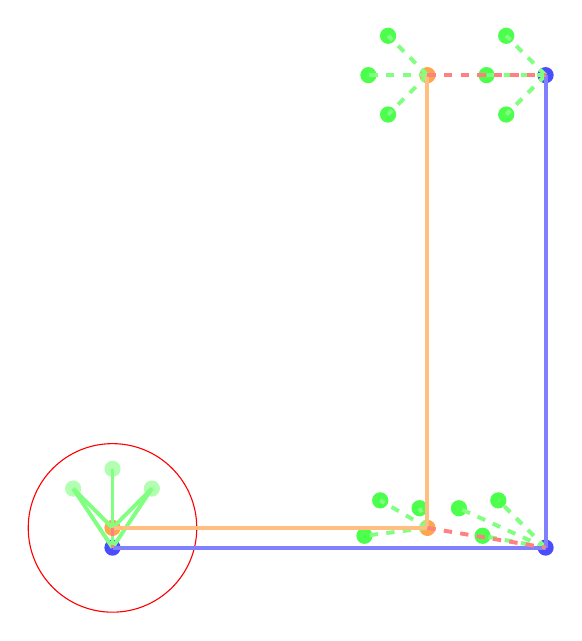
\begin{tikzpicture}
    \coordinate (A1) at (0, 0.25);
    \coordinate (A1MP1) at (-0.5, 0.75);
    \coordinate (A1MP2) at (0, 1.0);
    \coordinate (A1MP3) at (0.5, 0.75);

    \coordinate (B1) at (4, 0.25);
    \coordinate (B1MP1) at (3.2, 0.15);
    \coordinate (B1MP2) at (3.4, 0.6);
    \coordinate (B1MP3) at (3.9, 0.5);

    \coordinate (C1) at (4, 6);
    \coordinate (C1MP1) at (3.5, 6.5);
    \coordinate (C1MP2) at (3.25, 6.0);
    \coordinate (C1MP3) at (3.5, 5.5);

    \coordinate (A2) at (0, 0);

    \coordinate (B2) at (5.5, 0);
    \coordinate (B2MP1) at (4.7, 0.15);
    \coordinate (B2MP2) at (4.9, 0.6);
    \coordinate (B2MP3) at (4.4, 0.5);

    \coordinate (C2) at (5.5, 6);
    \coordinate (C2MP1) at (5.0, 6.5);
    \coordinate (C2MP2) at (4.75, 6.0);
    \coordinate (C2MP3) at (5.0, 5.5);

    \node [fill=orange!70, circle,inner sep=2pt, text width=0.1mm] at (A1) {};
    \node [fill=none, draw, red, circle, inner sep=2pt, text width=2.0cm] at (A1) {};
    \node [fill=green!30, circle,inner sep=2pt, text width=0.1mm] at (A1MP1) {};
    \node [fill=green!30, circle,inner sep=2pt, text width=0.1mm] at (A1MP2) {};
    \node [fill=green!30, circle,inner sep=2pt, text width=0.1mm] at (A1MP3) {};
    \draw [green!50, line width=0.05cm] (A1) to (A1MP1);
    \draw [green!50, line width=0.05cm] (A1) to (A1MP2);
    \draw [green!50, line width=0.05cm] (A1) to (A1MP3);

    \node [fill=orange!70, circle,inner sep=2pt, text width=0.1mm] at (B1) {};
    \node [fill=green!70, circle, inner sep=2pt, text width=0.1mm] at (B1MP1) {};
    \node [fill=green!70, circle, inner sep=2pt, text width=0.1mm] at (B1MP2) {};
    \node [fill=green!70, circle, inner sep=2pt, text width=0.1mm] at (B1MP3) {};
    \draw [green!50, dashed, line width=0.05cm] (B1) to (B1MP1);
    \draw [green!50, dashed, line width=0.05cm] (B1) to (B1MP2);
    \draw [green!50, dashed, line width=0.05cm] (B1) to (B1MP3);

    \node [fill=orange!70, circle,inner sep=2pt, text width=0.1mm] at (C1) {};
    \node [fill=green!70, circle, inner sep=2pt, text width=0.1mm] at (C1MP1) {};
    \node [fill=green!70, circle, inner sep=2pt, text width=0.1mm] at (C1MP2) {};
    \node [fill=green!70, circle, inner sep=2pt, text width=0.1mm] at (C1MP3) {};
    \draw [green!50, dashed, line width=0.05cm] (C1) to (C1MP1);
    \draw [green!50, dashed, line width=0.05cm] (C1) to (C1MP2);
    \draw [green!50, dashed, line width=0.05cm] (C1) to (C1MP3);

    \node [fill=blue!70, circle,inner sep=2pt, text width=0.1mm] at (A2) {};
    \draw [green!50, line width=0.05cm] (A2) to (A1MP1);
    \draw [green!50, line width=0.05cm] (A2) to (A1MP2);
    \draw [green!50, line width=0.05cm] (A2) to (A1MP3);

    \node [fill=blue!70, circle,inner sep=2pt, text width=0.1mm] at (B2) {};
    \node [fill=green!70, circle,inner sep=2pt, text width=0.1mm] at (B2MP1) {};
    \node [fill=green!70, circle,inner sep=2pt, text width=0.1mm] at (B2MP2) {};
    \node [fill=green!70, circle,inner sep=2pt, text width=0.1mm] at (B2MP3) {};
    \draw [green!50, dashed, line width=0.05cm] (B2) to (B2MP1);
    \draw [green!50, dashed, line width=0.05cm] (B2) to (B2MP2);
    \draw [green!50, dashed, line width=0.05cm] (B2) to (B2MP3);

    \node [fill=blue!70, circle,inner sep=2pt, text width=0.1mm] at (C2) {};
    \node [fill=green!70, circle, inner sep=2pt, text width=0.1mm] at (C2MP1) {};
    \node [fill=green!70, circle, inner sep=2pt, text width=0.1mm] at (C2MP2) {};
    \node [fill=green!70, circle, inner sep=2pt, text width=0.1mm] at (C2MP3) {};
    \draw [green!50, dashed, line width=0.05cm] (C2) to (C2MP1);
    \draw [green!50, dashed, line width=0.05cm] (C2) to (C2MP2);
    \draw [green!50, dashed, line width=0.05cm] (C2) to (C2MP3);

    \draw [orange!50, line width=0.05cm] (A1) to (B1);
    \draw [orange!50, line width=0.05cm] (B1) to (C1);
    \draw [blue!50, line width=0.05cm] (A2) to (B2);
    \draw [blue!50, line width=0.05cm] (B2) to (C2);

    \draw [red!50, line width=0.05cm, dashed] (A1) to (A2);
    \draw [red!50, line width=0.05cm, dashed] (B1) to (B2);
    \draw [red!50, line width=0.05cm, dashed] (C1) to (C2);
  \end{tikzpicture}
  \end{center}
}
\only<4>{
  Fuse map points in the $n-1$ keyframe matches
  \begin{center}
  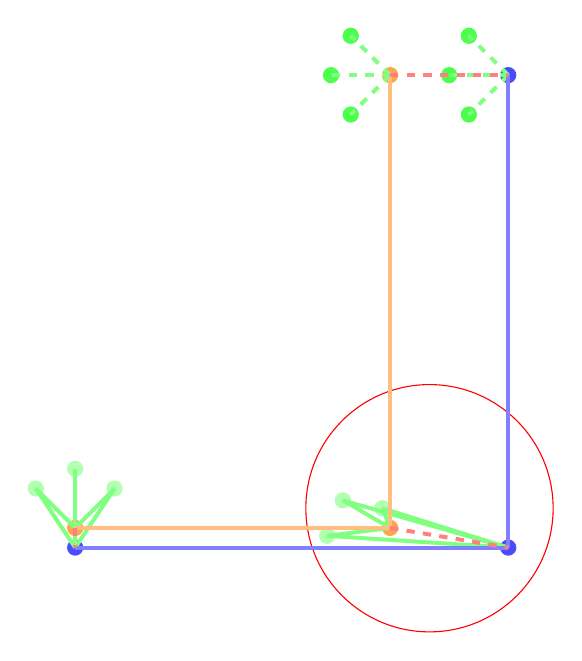
\begin{tikzpicture}
    \coordinate (A1) at (0, 0.25);
    \coordinate (A1MP1) at (-0.5, 0.75);
    \coordinate (A1MP2) at (0, 1.0);
    \coordinate (A1MP3) at (0.5, 0.75);

    \coordinate (B1) at (4, 0.25);
    \coordinate (B1MP1) at (3.2, 0.15);
    \coordinate (B1MP2) at (3.4, 0.6);
    \coordinate (B1MP3) at (3.9, 0.5);

    \coordinate (C1) at (4, 6);
    \coordinate (C1MP1) at (3.5, 6.5);
    \coordinate (C1MP2) at (3.25, 6.0);
    \coordinate (C1MP3) at (3.5, 5.5);

    \coordinate (A2) at (0, 0);
    
    \coordinate (B12) at (4.5, 0.5);
    \coordinate (B2) at (5.5, 0);

    \coordinate (C2) at (5.5, 6);
    \coordinate (C2MP1) at (5.0, 6.5);
    \coordinate (C2MP2) at (4.75, 6.0);
    \coordinate (C2MP3) at (5.0, 5.5);

    \node [fill=orange!70, circle,inner sep=2pt, text width=0.1mm] at (A1) {};
    \node [fill=green!30, circle,inner sep=2pt, text width=0.1mm] at (A1MP1) {};
    \node [fill=green!30, circle,inner sep=2pt, text width=0.1mm] at (A1MP2) {};
    \node [fill=green!30, circle,inner sep=2pt, text width=0.1mm] at (A1MP3) {};
    \draw [green!50, line width=0.05cm] (A1) to (A1MP1);
    \draw [green!50, line width=0.05cm] (A1) to (A1MP2);
    \draw [green!50, line width=0.05cm] (A1) to (A1MP3);

    \node [fill=orange!70, circle,inner sep=2pt, text width=0.1mm] at (B1) {};
    \node [fill=none, draw, red, circle, inner sep=2pt, text width=3.0cm] at (B12) {};
    \node [fill=green!30, circle, inner sep=2pt, text width=0.1mm] at (B1MP1) {};
    \node [fill=green!30, circle, inner sep=2pt, text width=0.1mm] at (B1MP2) {};
    \node [fill=green!30, circle, inner sep=2pt, text width=0.1mm] at (B1MP3) {};
    \draw [green!50, line width=0.05cm] (B1) to (B1MP1);
    \draw [green!50, line width=0.05cm] (B1) to (B1MP2);
    \draw [green!50, line width=0.05cm] (B1) to (B1MP3);

    \node [fill=orange!70, circle,inner sep=2pt, text width=0.1mm] at (C1) {};
    \node [fill=green!70, circle, inner sep=2pt, text width=0.1mm] at (C1MP1) {};
    \node [fill=green!70, circle, inner sep=2pt, text width=0.1mm] at (C1MP2) {};
    \node [fill=green!70, circle, inner sep=2pt, text width=0.1mm] at (C1MP3) {};
    \draw [green!50, dashed, line width=0.05cm] (C1) to (C1MP1);
    \draw [green!50, dashed, line width=0.05cm] (C1) to (C1MP2);
    \draw [green!50, dashed, line width=0.05cm] (C1) to (C1MP3);

    \node [fill=blue!70, circle,inner sep=2pt, text width=0.1mm] at (A2) {};
    \draw [green!50, line width=0.05cm] (A2) to (A1MP1);
    \draw [green!50, line width=0.05cm] (A2) to (A1MP2);
    \draw [green!50, line width=0.05cm] (A2) to (A1MP3);

    \node [fill=blue!70, circle,inner sep=2pt, text width=0.1mm] at (B2) {};
    \draw [green!50, line width=0.05cm] (B2) to (B1MP1);
    \draw [green!50, line width=0.05cm] (B2) to (B1MP2);
    \draw [green!50, line width=0.05cm] (B2) to (B1MP3);

    \node [fill=blue!70, circle,inner sep=2pt, text width=0.1mm] at (C2) {};
    \node [fill=green!70, circle, inner sep=2pt, text width=0.1mm] at (C2MP1) {};
    \node [fill=green!70, circle, inner sep=2pt, text width=0.1mm] at (C2MP2) {};
    \node [fill=green!70, circle, inner sep=2pt, text width=0.1mm] at (C2MP3) {};
    \draw [green!50, dashed, line width=0.05cm] (C2) to (C2MP1);
    \draw [green!50, dashed, line width=0.05cm] (C2) to (C2MP2);
    \draw [green!50, dashed, line width=0.05cm] (C2) to (C2MP3);

    \draw [orange!50, line width=0.05cm] (A1) to (B1);
    \draw [orange!50, line width=0.05cm] (B1) to (C1);
    \draw [blue!50, line width=0.05cm] (A2) to (B2);
    \draw [blue!50, line width=0.05cm] (B2) to (C2);

    \draw [red!50, line width=0.05cm, dashed] (A1) to (A2);
    \draw [red!50, line width=0.05cm, dashed] (B1) to (B2);
    \draw [red!50, line width=0.05cm, dashed] (C1) to (C2);
  \end{tikzpicture}
  \end{center}
}
\only<5>{
  Fuse map points in the $n-1$ keyframe matches
  \begin{center}
  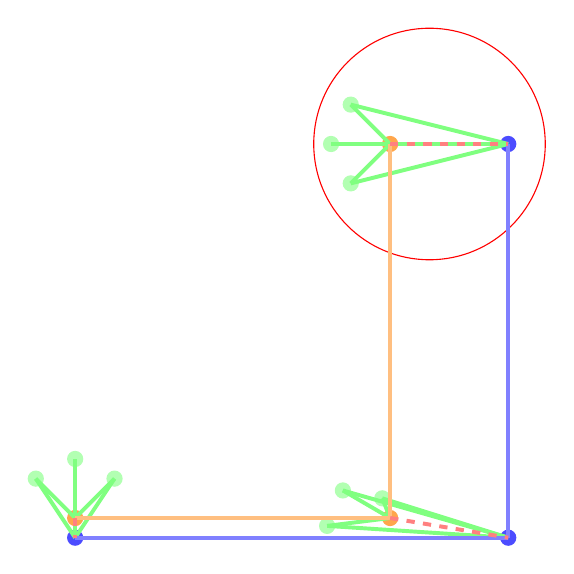
\begin{tikzpicture}
    \coordinate (A1) at (0, 0.25);
    \coordinate (A1MP1) at (-0.5, 0.75);
    \coordinate (A1MP2) at (0, 1.0);
    \coordinate (A1MP3) at (0.5, 0.75);

    \coordinate (B1) at (4, 0.25);
    \coordinate (B1MP1) at (3.2, 0.15);
    \coordinate (B1MP2) at (3.4, 0.6);
    \coordinate (B1MP3) at (3.9, 0.5);

    \coordinate (C1) at (4, 5);
    \coordinate (C1MP1) at (3.5, 5.5);
    \coordinate (C1MP2) at (3.25, 5.0);
    \coordinate (C1MP3) at (3.5, 4.5);

    \coordinate (A2) at (0, 0);

    \coordinate (B2) at (5.5, 0);

    \coordinate (C12) at (4.5, 5.0);
    \coordinate (C2) at (5.5, 5);

    \node [fill=orange!70, circle,inner sep=2pt, text width=0.1mm] at (A1) {};
    \node [fill=green!30, circle,inner sep=2pt, text width=0.1mm] at (A1MP1) {};
    \node [fill=green!30, circle,inner sep=2pt, text width=0.1mm] at (A1MP2) {};
    \node [fill=green!30, circle,inner sep=2pt, text width=0.1mm] at (A1MP3) {};
    \draw [green!50, line width=0.05cm] (A1) to (A1MP1);
    \draw [green!50, line width=0.05cm] (A1) to (A1MP2);
    \draw [green!50, line width=0.05cm] (A1) to (A1MP3);

    \node [fill=orange!70, circle,inner sep=2pt, text width=0.1mm] at (B1) {};
    \node [fill=green!30, circle, inner sep=2pt, text width=0.1mm] at (B1MP1) {};
    \node [fill=green!30, circle, inner sep=2pt, text width=0.1mm] at (B1MP2) {};
    \node [fill=green!30, circle, inner sep=2pt, text width=0.1mm] at (B1MP3) {};
    \draw [green!50, line width=0.05cm] (B1) to (B1MP1);
    \draw [green!50, line width=0.05cm] (B1) to (B1MP2);
    \draw [green!50, line width=0.05cm] (B1) to (B1MP3);

    \node [fill=orange!70, circle,inner sep=2pt, text width=0.1mm] at (C1) {};
    \node [fill=none, draw, red, circle, inner sep=2pt, text width=2.8cm] at (C12) {};
    \node [fill=green!30, circle, inner sep=2pt, text width=0.1mm] at (C1MP1) {};
    \node [fill=green!30, circle, inner sep=2pt, text width=0.1mm] at (C1MP2) {};
    \node [fill=green!30, circle, inner sep=2pt, text width=0.1mm] at (C1MP3) {};
    \draw [green!50, line width=0.05cm] (C1) to (C1MP1);
    \draw [green!50, line width=0.05cm] (C1) to (C1MP2);
    \draw [green!50, line width=0.05cm] (C1) to (C1MP3);

    \node [fill=blue!70, circle,inner sep=2pt, text width=0.1mm] at (A2) {};
    \draw [green!50, line width=0.05cm] (A2) to (A1MP1);
    \draw [green!50, line width=0.05cm] (A2) to (A1MP2);
    \draw [green!50, line width=0.05cm] (A2) to (A1MP3);

    \node [fill=blue!70, circle,inner sep=2pt, text width=0.1mm] at (B2) {};
    \draw [green!50, line width=0.05cm] (B2) to (B1MP1);
    \draw [green!50, line width=0.05cm] (B2) to (B1MP2);
    \draw [green!50, line width=0.05cm] (B2) to (B1MP3);

    \node [fill=blue!70, circle,inner sep=2pt, text width=0.1mm] at (C2) {};
    \draw [green!50, line width=0.05cm] (C2) to (C1MP1);
    \draw [green!50, line width=0.05cm] (C2) to (C1MP2);
    \draw [green!50, line width=0.05cm] (C2) to (C1MP3);

    \draw [orange!50, line width=0.05cm] (A1) to (B1);
    \draw [orange!50, line width=0.05cm] (B1) to (C1);
    \draw [blue!50, line width=0.05cm] (A2) to (B2);
    \draw [blue!50, line width=0.05cm] (B2) to (C2);

    \draw [red!50, line width=0.05cm, dashed] (A1) to (A2);
    \draw [red!50, line width=0.05cm, dashed] (B1) to (B2);
    \draw [red!50, line width=0.05cm, dashed] (C1) to (C2);
  \end{tikzpicture}
  \end{center}
}
\only<6>{
  \begin{block}{}
  \begin{itemize}
    \item Reducing risk of bad map merging as $n$ keyframe matches have to be found
    \item The fusion of the map points creates edges in the covisibility graph, which the pose graph optimization and the GBA can optimize.
    \item Pose graph optimization and GBA are performed for $n$ keyframe matches together -> Saves time
  \end{itemize}
  \end{block}
}
\end{frame}

%------------------------------------------------

%\begin{frame}
%\frametitle{Blocks of Highlighted Text}
%\begin{block}{Block 1}
%Lorem ipsum dolor sit amet, consectetur adipiscing elit. Integer lectus nisl, ultricies in feugiat rutrum, porttitor sit amet augue. Aliquam ut tortor mauris. Sed volutpat ante purus, quis accumsan dolor.
%\end{block}
%
%\begin{block}{Block 2}
%Pellentesque sed tellus purus. Class aptent taciti sociosqu ad litora torquent per conubia nostra, per inceptos himenaeos. Vestibulum quis magna at risus dictum tempor eu vitae velit.
%\end{block}
%
%\begin{block}{Block 3}
%Suspendisse tincidunt sagittis gravida. Curabitur condimentum, enim sed venenatis rutrum, ipsum neque consectetur orci, sed blandit justo nisi ac lacus.
%\end{block}
%\end{frame}

%------------------------------------------------

%\begin{frame}
%\frametitle{Multiple Columns}
%\begin{columns}[c] % The "c" option specifies centered vertical alignment while the "t" option is used for top vertical alignment
%
%\column{.45\textwidth} % Left column and width
%\textbf{Heading}
%\begin{enumerate}
%\item Statement
%\item Explanation
%\item Example
%\end{enumerate}
%
%\column{.5\textwidth} % Right column and width
%Lorem ipsum dolor sit amet, consectetur adipiscing elit. Integer lectus nisl, ultricies in feugiat rutrum, porttitor sit amet augue. Aliquam ut tortor mauris. Sed volutpat ante purus, quis accumsan dolor.
%
%\end{columns}
%\end{frame}

%------------------------------------------------
%\section{Project introduction}
%------------------------------------------------

%------------------------------------------------

% Showing position in presentation
%\begin{frame}
%  \frametitle{Overview}
%  \tableofcontents[currentsection]
%\end{frame}

%------------------------------------------------

%\begin{frame}
%\frametitle{Map Fusion for Collaborative UAV SLAM}
%\begin{block}{The goal}
%To develop a pipeline to merge maps created by different Unmanned Aerial Vehicles (UAVs) operating in the same area
%\end{block}
%\begin{block}{Usage}
%A common map is required for a team of UAVs to perform tasks, e.g. inspection, together.
%\end{block}
%\begin{table}
%\begin{tabular}{l l l}
%\toprule
%\textbf{Treatments} & \textbf{Response 1} & \textbf{Response 2}\\
%\midrule
%Treatment 1 & 0.0003262 & 0.562 \\
%Treatment 2 & 0.0015681 & 0.910 \\
%Treatment 3 & 0.0009271 & 0.296 \\
%\bottomrule
%\end{tabular}
%\caption{Table caption}
%\end{table}
%\end{frame}

%------------------------------------------------

%\begin{frame}
%\frametitle{Theorem}
%\begin{theorem}[Mass--energy equivalence]
%$E = mc^2$
%\end{theorem}
%\end{frame}

%------------------------------------------------

%\begin{frame}[fragile] % Need to use the fragile option when verbatim is used in the slide
%\frametitle{Verbatim}
%\begin{example}[Theorem Slide Code]
%\begin{verbatim}
%\begin{frame}
%\frametitle{Theorem}
%\begin{theorem}[Mass--energy equivalence]
%$E = mc^2$
%\end{theorem}
%\end{frame}\end{verbatim}
%\end{example}
%\end{frame}

%------------------------------------------------

%\begin{frame}
%\frametitle{Figure}
%Uncomment the code on this slide to include your own image from the same directory as the template .TeX file.
%%\begin{figure}
%%\includegraphics[width=0.8\linewidth]{test}
%%\end{figure}
%\end{frame}

%------------------------------------------------

%\begin{frame}[fragile] % Need to use the fragile option when verbatim is used in the slide
%\frametitle{Citation}
%An example of the \verb|\cite| command to cite within the presentation:\\~
%
%This statement requires citation \cite{p1}.
%\end{frame}

%------------------------------------------------

%\begin{frame}
%\frametitle{References}
%\footnotesize{
%\begin{thebibliography}{99} % Beamer does not support BibTeX so references must be inserted manually as below
%\bibitem[Smith, 2012]{p1} John Smith (2012)
%\newblock Title of the publication
%\newblock \emph{Journal Name} 12(3), 45 -- 678.
%\end{thebibliography}
%}
%\end{frame}

%------------------------------------------------

\begin{frame}
\Huge{\centerline{Thank you for your attention}}
\end{frame}

%----------------------------------------------------------------------------------------

\end{document}
